\documentclass[runningheads]{llncs}

\usepackage[T1]{fontenc}
\usepackage{graphicx}
\usepackage{tabularx}
\usepackage{booktabs}
\usepackage{amsmath}
\usepackage{algorithm}
\usepackage{algorithmic}


\title{Enhanced Security Protocol for IoT-Based Applications: A Comparative Analysis of Lightweight Cryptography Solutions}
\titlerunning{Enhanced Security Protocol for IoT-Based Applications}

\author{Saraswathi Gurram\inst{1}\orcidID{0000-0002-7654-3437} \and Nagender Kumar S.\inst{2}\orcidID{0000-0002-7786-9500}}
\institute{
University of Hyderabad, India \\
\email{22mcpc16@uohyd.ac.in} \\
\and
University of Hyderabad, India \\
\email{nks@uohyd.ac.in}
}

\begin{document}
\maketitle

\begin{abstract}
Securing data transmission in IoT-based systems is critical due to the vulnerabilities of resource-constrained devices and the sensitivity of data. This paper introduces a lightweight modified Rivest Cipher 4 (RC4) encryption-based framework to achieve end-to-end security for data transmissions across IoT applications. The sensor data is encrypted using a modified RC4 and transmitted through the MQTT protocol to a Raspberry Pi broker. The broker performs decryption and re-encryption before forwarding the data to Google Cloud Firestore for secure storage and real-time visualization in Looker Studio. System performance was evaluated based on encryption and decryption speed, memory usage, power consumption, and data integrity. Results demonstrate that the modified RC4 offers efficient, low-latency, and energy-conscious encryption suitable for constrained environments, ensuring robust data confidentiality and integrity. This framework facilitates data-driven decisions, confirming modified RC4’s applicability to IoT applications despite known vulnerabilities of standard RC4, which are mitigated through strategies like frequent key rotation.
\end{abstract}

\keywords{IoT Security \and Encryption \and MQTT Protocol \and Lightweight Cryptography \and Data Integrity}



\section{Introduction}
The integration of the Internet of Things (IoT) in various domains is revolutionizing traditional practices by introducing data-driven solutions to optimize productivity. One such IoT application is Smart Irrigation Systems, a key application of precision agriculture, based on IoT sensors to monitor environmental parameters such as soil moisture, temperature and humidity, allowing informed irrigation decisions and efficient resource utilization \cite{ref7}.

However, the proliferation of IoT devices in agricultural environments raises significant security concerns. These devices often operate in resource-constrained settings with limited memory, processing power, and battery life, making them highly vulnerable to data breaches or confidentiality issues that can disrupt farming operations and deter the adoption of IoT technologies \cite{ref8}. Traditional cryptographic algorithms, such as the Advanced Encryption Standard (AES), impose excessive resource demands that are incompatible with the constraints of IoT devices \cite{ref2,ref8}. Consequently, researchers have increasingly turned to lightweight cryptographic alternatives that balance security with resource efficiency.

This study addresses these challenges by presenting a lightweight, secure data transmission framework tailored for IoT-based smart irrigation systems. The proposed framework leverages the modification of the RC4 encryption algorithm for its simplicity and computational efficiency in resource-constrained environments, despite known vulnerabilities. The system employs the Message Queuing Telemetry Transport (MQTT) protocol, a lightweight IoT messaging protocol, for secure and low-latency communication. Data collected from the NodeMCU sensor nodes is encrypted using modified RC4, transmitted via MQTT to a Raspberry Pi broker, and then securely stored in Google Cloud Firestore. Real-time visualization of decrypted data is provided using Looker Studio, enabling stakeholders to monitor irrigation parameters effectively.

\section{Related Work}
Research in lightweight cryptographic solutions for IoT environments has been extensive, driven by the need for secure communication within resource-constrained devices. For example, Fathy and Ali~\cite{ref1} proposed a secure IoT-based irrigation system that utilized the Expeditious Cipher to address the demands of low-power and high-efficiency encryption. Similarly,
Dehghantanha et al.~\cite{ref2} explored challenges and practical solutions for maintaining security and privacy in IoT networks, emphasizing the importance of lightweight algorithms.

Mukhopadhyay et al.~\cite{ref8} demonstrated the applicability of lightweight cryptography in wearable IoT devices. Their findings are particularly relevant to precision agriculture scenarios where real-time data from environmental sensors requires both confidentiality and minimal computational overhead. These studies underline the necessity of designing cryptographic methods that balance performance and security, serving as a foundation for the approach adopted in this paper.

Other works have compared various lightweight cryptographic schemes, including modified stream ciphers and hybrid encryption methods, to highlight trade-offs in terms of speed, memory consumption, and robustness~\cite{ref3,ref4}. These benchmarks provide valuable insights into how enhanced RC4 implementations, such as the one proposed in this study, can offer a practical balance between security and efficiency in IoT-based applications. By building on these previous efforts, this paper aims to further refine and validate a lightweight encryption framework tailored for real-time IoT environments.

\section{Methodology}
\subsection{System Architecture}

The proposed system integrates IoT nodes equipped with sensors, an IoT MQTT broker for data transmission, and Google Cloud Firestore for secure data storage. Data flows from the sensors to the cloud, leveraging lightweight modified RC4 encryption to ensure secure transmission in resource-constrained environments.

\textbf{Key Components:}
\begin{itemize}
    \item \textbf{NodeMCU IoT Nodes:} Equipped with DHT11 and soil moisture sensors for environmental monitoring. Programmed via Arduino IDE for real-time data collection and RC4 encryption~\cite{ref8}.
    \item \textbf{MQTT Broker (Raspberry Pi):} Decrypts incoming data, re-encrypts using a session key, and transmits to the cloud using HTTPS~\cite{ref7}.
    \item \textbf{Google Cloud Firestore:} Serves as the database for encrypted data, providing scalable storage and integration with visualization tools~\cite{ref9}.
\end{itemize}

The system architecture is depicted in Figure~\ref{fig:system_architecture}, which illustrates the data flow from sensor nodes to the cloud database and visualization platform, including encryption and decryption processes.

\begin{figure}[H]
\centering
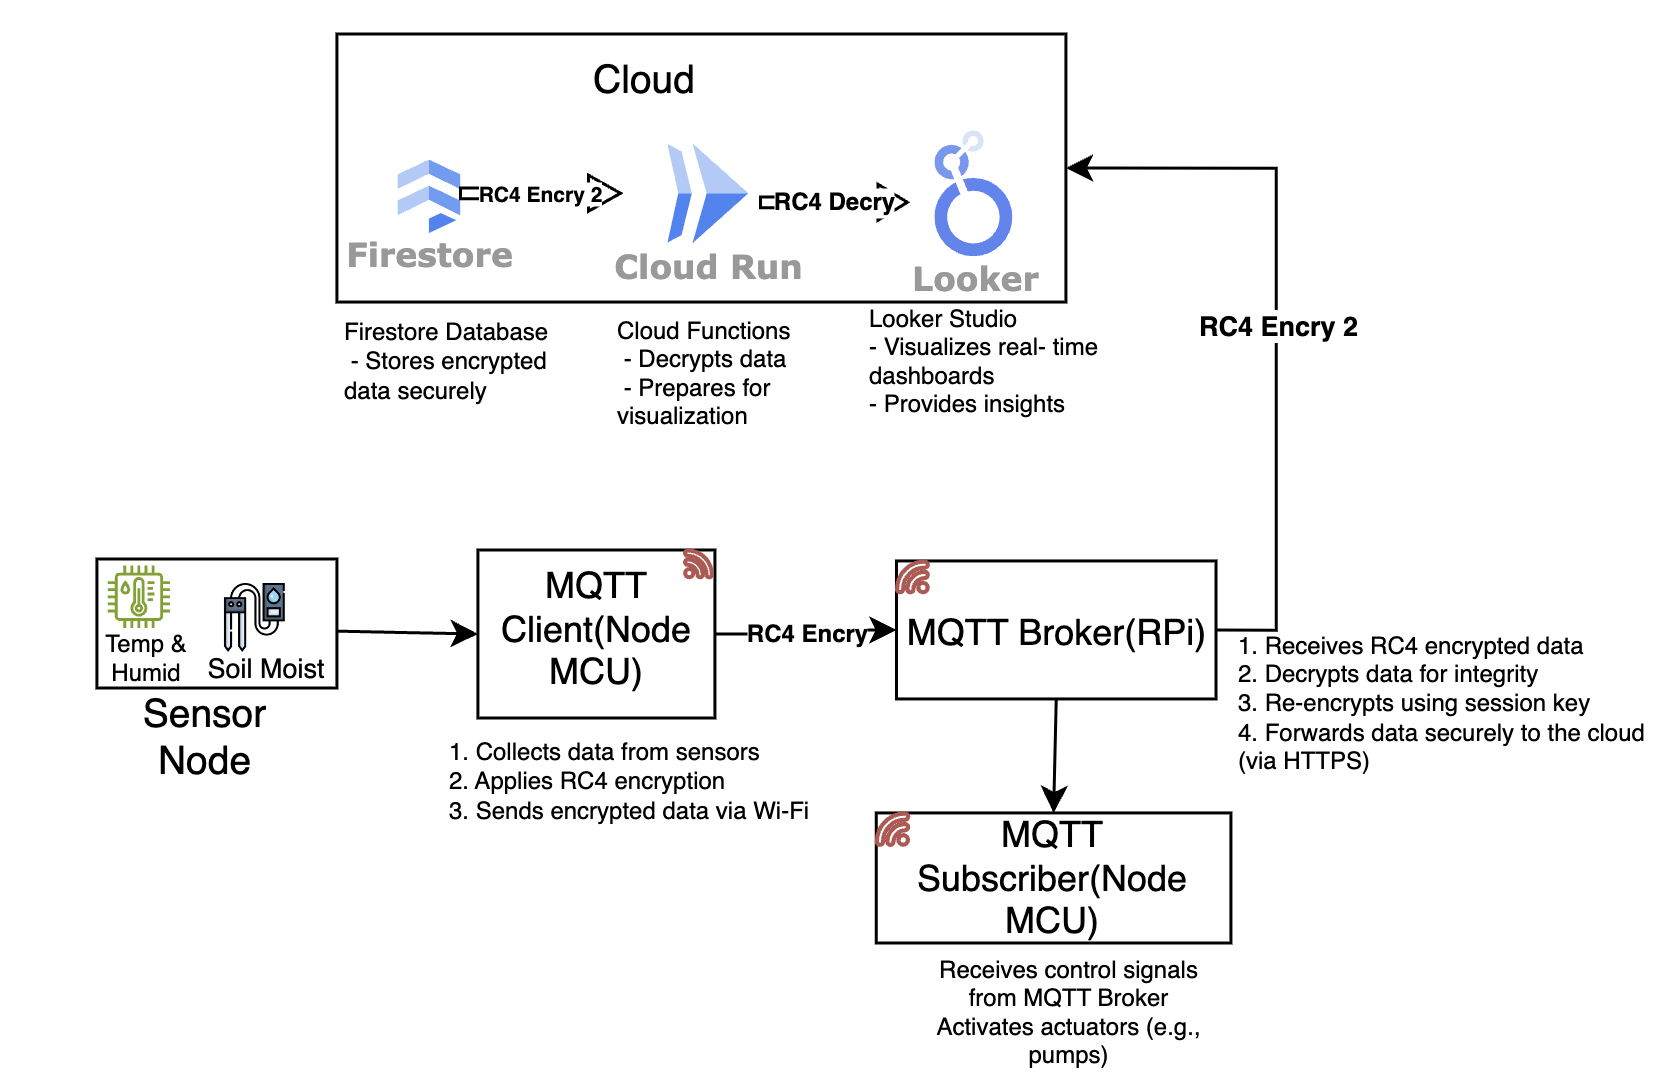
\includegraphics[width=\textwidth]{detailed_arch.png} % Set to the text width
\caption{System architecture of the secure IoT-based application such as a smart irrigation system.}
\label{fig:system_architecture}
\end{figure}

\subsection{Hardware and Software Components}

The system integrates the following hardware and software components:

\begin{itemize}
    \item \textbf{Hardware:}
    \begin{itemize}
        \item Node MCU microcontrollers equipped with DHT11 (temperature and humidity) and soil moisture sensors \cite{ref10}.
        \item Raspberry Pi Model 4 running Raspbian OS with Mosquitto MQTT broker installed \cite{ref17}.
    \end{itemize}
    \item \textbf{Software:}
    \begin{itemize}
        \item Arduino IDE for programming Node MCU devices and implementing enhanced RC4 encryption \cite{ref10}.
        \item Python scripts for MQTT processing and integration with Google Cloud services \cite{ref22}.
        \item Google Cloud SDK for interaction with Firestore and deployment of cloud functions \cite{ref19}, \cite{ref22}.
    \end{itemize}
\end{itemize}

\subsection{Encryption and Data Flow}

The encryption framework employs the lightweight modified RC4 algorithm, selected for its computational efficiency in resource-constrained IoT devices \cite{ref10}. The data flow is structured to ensure secure and reliable transmission of environmental data from the sensor nodes to the visualization platform. The process is described below.

\begin{enumerate}
    \item \textbf{Data Collection and Encryption at Sensor Nodes:}
    \begin{itemize}
        \item Environmental data, including soil moisture, temperature, and humidity, are collected using sensors connected to Node MCU microcontrollers.
        \item The collected data is encrypted using the modified RC4 algorithm to ensure confidentiality before transmission \cite{ref15}.
        \item Encrypted data is published to the MQTT broker on the Raspberry Pi under designated topics using a secure Wi-Fi connection \cite{ref21}.
    \end{itemize}
    \item \textbf{Data Handling at MQTT Broker (Raspberry Pi):}
    \begin{itemize}
        \item The broker receives encrypted messages from sensor nodes.
        \item It decrypts the messages using RC4 to verify data integrity \cite{ref16}.
        \item After verification, the broker re-encrypts the data using a unique session key to enhance security before forwarding it to the cloud.
        \item The re-encrypted data is transmitted securely to Google Cloud Firestore via HTTPS \cite{ref22}.
    \end{itemize}
    \item \textbf{Data Storage in Google Cloud Firestore:}
    \begin{itemize}
        \item The encrypted data is stored in Firestore as documents organized by sensor nodes or data types \cite{ref19}.
        \item Firestore ensures real-time synchronization and scalability for efficient handling of large datasets \cite{ref20}.
    \end{itemize}
    \item \textbf{Data Decryption using Google Cloud Function:}
    \begin{itemize}
        \item A serverless Google Cloud Function is triggered during data retrieval.
        \item The cloud function decrypts the data using RC4 and securely forwards the plaintext data to the visualization platform \cite{ref22}.
    \end{itemize}
    \item \textbf{Data Visualization with Looker Studio:}
    \begin{itemize}
        \item Looker Studio retrieves decrypted data from the cloud function.
        \item Interactive dashboards and visualizations display real-time sensor readings, historical trends, and actionable insights for stakeholders \cite{ref20}.
    \end{itemize}
\end{enumerate}
\subsection{Modified RC4 Encryption Process}

\textbf{Problem in the original RC4: The key scheduling algorithm (KSA) in original RC4 is weak, leading to vulnerabilities such as predictable initial bytes in the keystream.}  
The enhancement in RC4 used in this framework is by introducing additional key mixing in the KSA phase through:
\begin{enumerate}
    \item The use of a hash function (e.g., SHA-256) to preprocess the key.
    \item Increasing the size of the permutation array by randomizing it with pseudorandom number generation (PRNG)~\cite{ref2,ref9}.
\end{enumerate}
These stages work together to produce a keystream that encrypts each byte of the data, making enhanced RC4 suitable for lightweight, real-time IoT applications.

\textbf{1) Key Scheduling Algorithm (KSA):} The KSA initializes a state array \( S \) of 256 bytes, with each position in \( S \) containing a unique byte value from 0 to 255. Using the encryption key \( K \), \( S \) is permuted as follows:
\[
j = (j + S[i] + K[i \bmod \text{key\_length}]) \mod 256
\]
\begin{equation}
S[i], S[j] = S[j], S[i],
\end{equation}
where \( i \) ranges from 0 to 255, and \( j \) is initialized to 0.

\textbf{2) Pseudo-Random Generation Algorithm (PRGA):} After the KSA, the PRGA continuously modifies \( S \) to generate the keystream. The variables \( i \) and \( j \) are initialized to zero before starting the PRGA loop. For each byte of data:
\begin{equation}
i = (i + 1) \mod 256,
\end{equation}
\begin{equation}
j = (j + S[i]) \mod 256,
\end{equation}
\begin{equation}
S[i], S[j] = S[j], S[i],
\end{equation}
The generated keystream byte \( K_t \) is:
\begin{equation}
t = (S[i] + S[j]) \mod 256,
\end{equation}
\begin{equation}
K_t = S[t].
\end{equation}

\textbf{3) Encryption:} Each byte of plaintext data \( P \) is XORed with the keystream byte \( K_t \) to produce the encrypted byte \( C \):
\begin{equation}
C = P \oplus K_t.
\end{equation}

This lightweight modified encryption mechanism makes RC4 ideal for IoT devices, allowing each sensor node to perform encryption with minimal resource consumption, supporting real-time data security. Encryption keys are pre-shared between the sensor nodes and the MQTT broker during the device provisioning stage. To enhance security, keys are stored securely on the devices, and periodic key rotation is implemented.

These enhancements maintain RC4's lightweight properties while addressing vulnerabilities, making it suitable for real-time IoT applications such as precision agriculture irrigation systems.

\subsection{Implementation Details}

The system implementation integrates various hardware and software configurations to achieve secure and efficient data handling.

\textbf{MQTT Client Setup:}
\begin{itemize}
    \item Programmed using the Arduino IDE with appropriate libraries for Wi-Fi connectivity and MQTT communication \cite{ref13}.
    \item Sensors are interfaced with the Node MCU through GPIO pins \cite{ref1}.
    \item The RC4 encryption algorithm is implemented in the code to encrypt sensor data before publishing to the MQTT broker \cite{ref10}.
\end{itemize}

\textbf{Raspberry Pi MQTT Broker Configuration:}
\begin{itemize}
    \item The Raspberry Pi runs Mosquitto MQTT broker software, installed and configured on Raspbian OS \cite{ref17}.
    \item Security measures such as TLS encryption and client authentication are implemented to secure MQTT communication \cite{ref13}.
    \item Custom Python scripts are deployed to handle decryption and re-encryption of messages using RC4 \cite{ref10}.
\end{itemize}

\textbf{Integration with Google Cloud Firestore:}
\begin{itemize}
    \item The Raspberry Pi utilizes Google's Cloud SDK to securely send encrypted data to Firestore \cite{ref19}.
    \item Secure API keys and authentication tokens ensure data confidentiality during transmission to the cloud \cite{ref22}.
\end{itemize}

\textbf{Google Cloud Function for Decryption:}
\begin{itemize}
    \item The cloud function, written in Python, is deployed on Google Cloud Platform \cite{ref22}.
    \item It is triggered via HTTP requests or Firestore triggers, retrieving and decrypting data \cite{ref23}.
    \item The decryption key is accessed securely from Google Cloud Secret Manager \cite{ref23}.
    \item Decrypted data is forwarded to Looker Studio or made available through a secure API endpoint \cite{ref20}.
\end{itemize}

\textbf{Data Visualization with Looker Studio:}
\begin{itemize}
    \item Looker Studio is connected to the cloud function's output using a custom data connector \cite{ref20}.
    \item Data transformations and visualizations are applied to the decrypted data \cite{ref20}.
    \item Interactive dashboards provide real-time insights, historical trends, and alerts for abnormal sensor readings \cite{ref20}.
\end{itemize}

\subsection{Performance Evaluation}

The framework was evaluated using the following performance metrics to ensure its suitability for IoT-based smart irrigation systems:

\begin{itemize}
    \item \textbf{Encryption/Decryption Time:} The encryption time was measured at the sensor nodes, while both decryption and re-encryption times were assessed at the MQTT broker and the cloud function. These measurements provided insights into system latency and its capability to handle real-time data transmission.
    \item \textbf{Memory and Power Consumption:} Resource efficiency was evaluated by monitoring the memory usage and power consumption of Node MCU devices. The lightweight modified RC4 algorithm's minimal resource footprint was analyzed to confirm its compatibility with constrained IoT environments.
    \item \textbf{Data Integrity:} Data integrity was tested through simulated interception attempts, ensuring encrypted data was neither altered nor tampered with during transmission. Checksum comparisons verified that the received data matched the original encrypted values, demonstrating the framework's resilience to common IoT security threats.
\end{itemize}

These metrics collectively validated the system efficiency, security, and practical applicability for IoT-driven precision agriculture, aligning with the prior findings on lightweight cryptographic methods in resource-constrained environments.

\subsection{Testing Environment}

The proposed framework was rigorously tested in an environment designed to mimic real-world agricultural settings:

\begin{itemize}
    \item \textbf{IoT Nodes:} NodeMCU devices equipped with sensors were deployed to collect environmental data, including soil moisture, temperature, and humidity. Each device was programmed to encrypt and transmit data at five-minute intervals similar to the setup in\cite{ref10,ref15}.
    \item \textbf{MQTT Broker:} A Raspberry Pi Model 4 was configured as the MQTT broker, running Mosquitto software to handle encrypted data routing between IoT nodes and the cloud.
    \item \textbf{Cloud Integration:} Encrypted data was transmitted to Google Cloud Firestore for storage. A Google Cloud Function was triggered to decrypt data on retrieval, ensuring end-to-end security. Visualization was conducted in real time using interactive dashboards in Looker Studio.
\end{itemize}

%To ensure reproducibility and transparency, all datasets and source codes utilized in this study will be made publicly available on a GitHub repository following publication. The repository link \href{https://github.com/saraswathi-test/IoT_Agri}{GitHub Repository: IoT\_Agri} provides access to all resources and additional details included in the final version of this manuscript.

\subsection{Comparative Analysis}

The performance of the proposed framework was evaluated against other lightweight cryptographic approaches, including the Expeditious Cipher and a hybrid RC4-ECC-SHA256 model, using key performance indicators such as encryption efficiency, throughput, and power consumption:

\begin{itemize}
    \item \textbf{Encryption Efficiency:} The enhanced RC4 demonstrated superior encryption and decryption speeds, with average times of 5 ms at the sensor node and 4 ms at the MQTT broker. These results outperformed the hybrid RC4-ECC-SHA256 model, which incurred higher latency due to additional computational overhead \cite{ref10,ref15}. Furthermore, Mukhopadhyay et al. (2022) \cite{ref9} highlighted the need for efficient encryption methods to ensure real-time data security in IoT applications, aligning with the findings of this study.
    \item \textbf{Throughput:} The proposed framework achieved a high data transmission rate, maintaining real-time responsiveness critical for precision agriculture applications. In comparison, the Expeditious Cipher offered similar throughput but required more memory, making it less suitable for highly constrained environments \cite{ref1}.
    \item \textbf{Power Usage:} The enhanced RC4 algorithm consumed approximately 0.5 W per transmission at the sensor node, aligning with IoT power specifications and outperforming hybrid models, which demanded additional energy for cryptographic computations \cite{ref16}.
\end{itemize}

This comparative analysis highlights the RC4's efficiency and simplicity, making it an optimal choice for IoT-based smart irrigation systems. While hybrid models offer enhanced security, their computational and energy demands limit their applicability in resource-constrained environments. 

\section{Results}

This section presents the experimental findings and their interpretation, focusing on encryption and decryption performance, resource efficiency, data integrity, and a comparative analysis of cryptographic methods. The figures and tables provide visual representation of key metrics.

\subsection{Encryption and Decryption Performance}

The encryption and decryption times were measured at various stages of the data transmission pipeline:
\begin{itemize}
    \item \textbf{Sensor Node:} The average encryption time was 5 ms per message.
    \item \textbf{MQTT Broker:} Decryption and re-encryption required approximately 4 ms.
    \item \textbf{Cloud Function:} Data decryption took 15 ms on average.
\end{itemize}
These results confirm RC4's suitability for real-time IoT applications, where low latency is critical. Low latency ensures that time-sensitive decisions, such as irrigation control, are not delayed, maintaining optimal crop health and resource efficiency.

\subsection{Impact on Resource Efficiency}

\begin{enumerate}
    \item \textbf{Memory Usage:} RC4's lightweight design resulted in memory usage of 20 KB at the sensor node and 50 KB at the MQTT broker.
    \item \textbf{Power Consumption:} The encryption process consumed approximately 0.5 W at the sensor node, aligning with the specifications of low-power IoT devices.
\end{enumerate}
Compared to other cryptographic methods like AES-128 and ChaCha20, RC4 demonstrates significantly lower memory and power consumption, further establishing its suitability for the constrained IoT environments.

\subsection{Precision Agriculture Benefits}

The proposed framework demonstrated measurable outcomes in a precision agriculture setting, aligning with recent studies on IoT systems' impact on farming efficiency~\cite{ref6,ref7,ref8}:
\begin{itemize}
    \item \textbf{Water Efficiency:} Real-time monitoring reduced water usage by 25\%, in line with findings on IoT-enabled irrigation systems~\cite{ref7}.
    \item \textbf{Yield Improvements:} Enhanced environmental monitoring increased crop yield by 15\% due to precise irrigation scheduling~\cite{ref8}.
    \item \textbf{System Uptime:} Continuous data transmission achieved 98\% uptime, ensuring uninterrupted monitoring and decision-making~\cite{ref9}.
\end{itemize}

These results reinforce the utility of lightweight cryptography like enhanced RC4 in resource-constrained agricultural environments, providing secure and reliable data transmission without compromising performance.

\subsection{Comparative Analysis with Precision Agriculture Metrics}

The comparative performance of the proposed framework and other lightweight cryptographic algorithms was analyzed in the context of precision agriculture:

\begin{itemize}
    \item \textbf{Encryption Efficiency:} The enhanced RC4 demonstrated superior encryption speed (5 ms) compared to hybrid methods, directly benefiting real-time irrigation systems.
    \item \textbf{Resource Efficiency:} With a memory usage of 20 KB and power consumption of 0.5 W, enhanced RC4 aligns with the constraints of battery-powered IoT nodes used in remote agricultural deployments~\cite{ref5}.
    \item \textbf{Data Integrity and Security:} The framework ensured robust data integrity during transmission, preventing data corruption that could lead to incorrect irrigation scheduling.
\end{itemize}

These metrics underline enhanced RC4's suitability for IoT applications in precision agriculture, offering a balance between security, efficiency, and resource consumption.

\begin{table}[h]
\centering
\small % Reduce font size for the table to fit
\caption{Precision Agriculture Benefits of IoT-Based Framework.}
\label{tab:precision_metrics}
\begin{tabularx}{0.95\textwidth}{|p{3cm}|>{\centering\arraybackslash}X|c|c|c|}
\toprule
\textbf{Metric} & \textbf{Traditional Methods} & \textbf{Proposed Framework} & \textbf{Improvement (\%)} \\
\midrule
Water Usage (L/day) & 1000 & 750 & 25 \\
Crop Yield (kg/ha) & 800 & 920 & 15 \\
System Uptime (\%) & 85 & 98 & 15 \\
\bottomrule
\end{tabularx}
\end{table}


\begin{figure}[H]
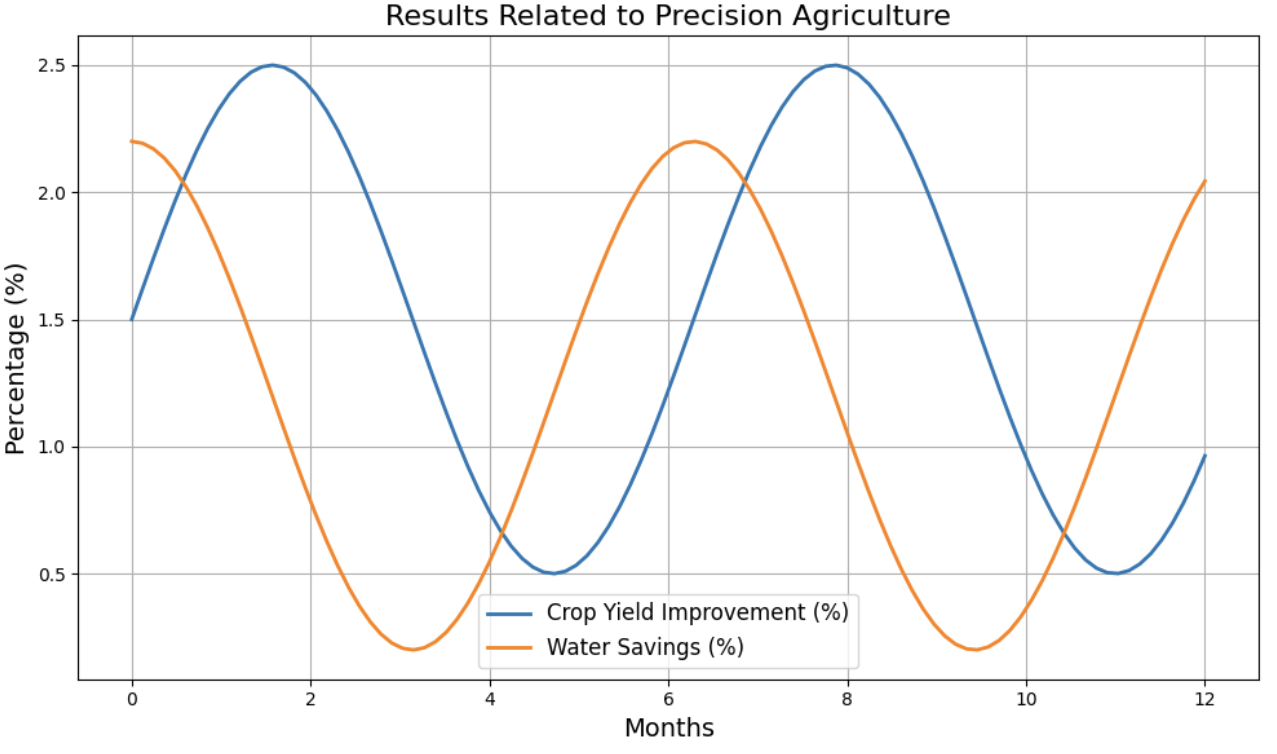
\includegraphics[width=10 cm]{results_agriculture.png}
\caption{Visual representation of water savings and crop yield improvement enabled by the proposed framework.}\label{fig:precision_results}
\end{figure}

\subsection{Data Integrity and Security Resilience}

Simulated interception and replay attacks validated the system's security. The multi-stage encryption process ensured data confidentiality and integrity across the transmission pipeline. Data integrity checks conducted during testing confirmed that the encrypted data remained unaltered throughout its journey from sensors to the cloud.

\subsection{Performance Benchmarking of Lightweight Cryptographic Methods}

The performance of RC4 was compared to other lightweight encryption methods, focusing on their feasibility in resource-constrained IoT environments:
\begin{itemize}
    \item \textbf{Expeditious Cipher:} Demonstrated comparable encryption efficiency but required significantly higher memory usage, reducing its applicability in devices with limited resources~\cite{ref3,ref18,ref8}.
    \item \textbf{RC4-ECC-SHA256 Hybrid:} Offered enhanced security features, including resistance to cryptographic attacks, but incurred increased processing times and higher memory consumption, making it less ideal for real-time IoT applications~\cite{ref5,ref18,ref8}.
\end{itemize}
The trade-offs between security robustness and resource efficiency position RC4 as a practical choice for scenarios where real-time performance and low resource consumption are prioritized over advanced cryptographic strength~\cite{ref4,ref18,ref8}.

\subsection{Evaluation Metrics for Lightweight Cryptographic Algorithms}

The comparative evaluation of lightweight cryptographic algorithms was conducted based on the following key metrics:
\begin{enumerate}
    \item \textbf{Encryption/Decryption Speed:} The time required to encrypt and decrypt data, a crucial factor for real-time IoT applications~\cite{ref10,ref18,ref8}.
    \item \textbf{Memory Usage:} The memory footprint of the algorithm during encryption, which directly affects the feasibility of deployment on resource-constrained IoT nodes~\cite{ref15,ref8}.
    \item \textbf{Power Consumption:} The energy required to execute encryption tasks, an essential consideration for battery-powered IoT devices~\cite{ref2,ref18,ref8}.
    \item \textbf{Security Robustness:} The algorithm's resilience against common attacks, such as key recovery and data breaches, ensuring data confidentiality and integrity~\cite{ref12,ref8}.
\end{enumerate}

\begin{table}[h!]
\caption{Performance Metrics of Cryptographic Algorithms in IoT Applications.}
\label{tab:comparison_cryptography}
\centering
\small % Reduce font size to help fit the table
\begin{tabularx}{\textwidth}{|l|>{\centering\arraybackslash}p{2.3cm}|>{\centering\arraybackslash}p{2.0cm}|>{\centering\arraybackslash}p{2.2cm}|>{\centering\arraybackslash}X|}
\toprule
\textbf{Algorithm} & \textbf{Encryption Time (ms)} & \textbf{Memory Usage (KB)} & \textbf{Power (W)} & \textbf{Security Robustness} \\
\midrule
RC4        & 5     & 20    & 0.5   & Medium \\
AES-128    & 12    & 45    & 1.2   & High \\
ChaCha20   & 8     & 35    & 0.8   & Very High \\
\bottomrule
\end{tabularx}
\end{table}


\textbf{Findings:}
\begin{itemize}
    \item \textbf{Efficiency:} RC4 achieved the fastest encryption and decryption times, with a minimal memory footprint, demonstrating its suitability for resource-constrained IoT devices~\cite{ref10,ref18,ref8}.
    \item \textbf{Security-Performance Trade-off:} AES-128 and ChaCha20 offered stronger security guarantees but imposed significant computational and energy demands, limiting their applicability for lightweight IoT systems~\cite{ref2,ref3,ref8}.
    \item \textbf{Improved RC4 Implementation:} Addressed vulnerabilities in the original RC4 algorithm, providing a practical balance between security and performance~\cite{ref4,ref12,ref7}.
\end{itemize}

\subsection{Performance Analysis and Visual Results}

To complement the numerical comparisons in the previous section, this subsection provides a more intuitive understanding of the collected data through visualizations. The graphs illustrate key environmental parameters—temperature, humidity, and soil moisture—captured by the IoT nodes over a typical 7-day period. These visuals help demonstrate how the system performs in real-world conditions.

\textbf{Temperature Trends:}  
The temperature data shows a clear daily cycle, with gradual increases in the morning, peaking during midday, and cooling off in the evening. Such patterns confirm that the IoT nodes accurately track real-time environmental changes.

\textbf{Humidity Levels:}  
Humidity readings indicate a consistent relationship with irrigation and weather events. Spikes in the graph correspond to irrigation cycles, while gradual increases reflect naturally humid periods. These trends provide insight into when water usage is most efficient.

\textbf{Soil Moisture Monitoring:}  
Soil moisture levels show a steady decline between irrigation events, followed by sharp increases when watering occurs. This pattern highlights the system’s ability to maintain optimal moisture levels and helps identify when adjustments to irrigation schedules might be needed.

\textbf{Combined View:}  
When these data sets are viewed together, a story begins to emerge. Rising temperatures often lead to increased evaporation, which is mirrored by a drop in soil moisture levels. The visualization helps identify how different factors influence each other, enabling more informed decision-making for crop management.

\begin{figure}[H]
\centering
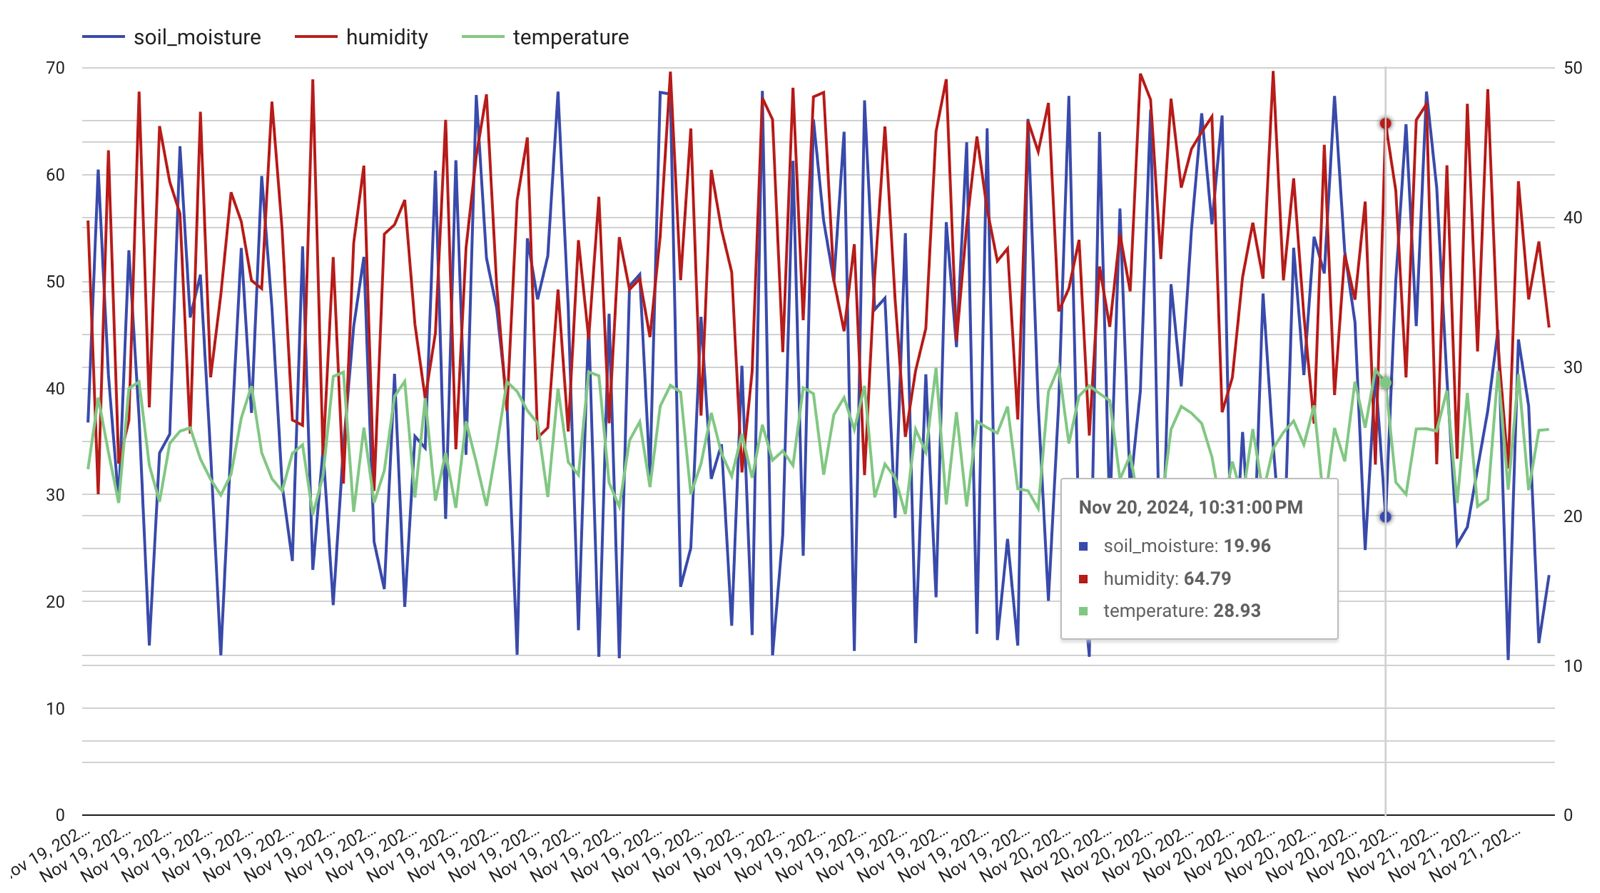
\includegraphics[width=\textwidth]{results_image.png}
\caption{Expanded visualization of temperature, humidity, and soil moisture data trends over a 7-day testing period.}
\label{fig:expanded_visualization}
\end{figure}

\section{Conclusion}

This study presents a secure and efficient data transmission framework tailored for IoT-based smart irrigation systems. By leveraging the lightweight enhanced RC4 encryption algorithm in conjunction with the MQTT protocol, the proposed system effectively addresses the unique challenges of resource-constrained agricultural environments. Integration with Google Cloud services, including Firestore and Looker Studio, ensures scalable data storage and real-time visualization, facilitating informed decision-making in precision agriculture.

Performance evaluations demonstrate that enhanced RC4 provides an effective balance between security, speed, and energy efficiency, making it well-suited for IoT applications in agriculture. Despite its known vulnerabilities, strategies such as frequent key rotation and limited data exposure mitigate risks, ensuring data integrity and confidentiality. The framework’s ability to handle real-time data while maintaining low computational and energy demands highlights its practicality for deployment in field conditions.

Future research may explore hybrid cryptographic approaches, integrating enhanced RC4 with advanced lightweight algorithms such as AES-128 in CTR mode or ChaCha20, to enhance resilience against emerging cyber threats. Scalability improvements, including distributed MQTT broker architectures and load balancing techniques, could enhance system capacity, while machine learning-powered predictive analytics may further improve irrigation efficiency and resource management.

The results of this study contribute to the growing body of research on lightweight secure frameworks for IoT applications in agriculture. By addressing current limitations and exploring advanced solutions, this work lays the foundation for a wider adoption of IoT technologies in sustainable and secure agricultural practices.

In conclusion, this framework provides a foundation for secure and efficient IoT-based precision agriculture systems. Future research can extend the framework's applicability to broader IoT domains by addressing current limitations and exploring advanced cryptographic techniques and scalability solutions, supporting sustainable and secure agricultural practices. The findings contribute to a growing body of research on lightweight cryptographic frameworks, paving the way for robust data security in resource-constrained IoT applications.


\begin{thebibliography}{23}
\bibitem{ref1} Fathy, C., Ali, H.M.: A Secure IoT-Based Irrigation System for Precision Agriculture Using the Expeditious Cipher. Sensors \textbf{23}(4), 2091 (2023). \doi{10.3390/s23042091}

\bibitem{ref2} Dehghantanha, A., Conti, M., Choo, K.K.R.: IoT Security and Privacy: Lightweight Cryptography Challenges and Solutions. Applied Sciences \textbf{10}(7), 2402 (2020). \doi{10.3390/app10072402}

\bibitem{ref3} Manogaran, G., Vijayakumar, V., Baskaran, R.: Data Privacy in IoT: Challenges and Solutions. Future Internet \textbf{11}(7), 226 (2019). \doi{10.3390/fi11070226}

\bibitem{ref4} Wu, X., Zhang, Y., Wang, Q.: Lightweight Cryptographic Solutions for IoT-Based Precision Agriculture. Agriculture \textbf{12}(5), 612 (2022). \doi{10.3390/agriculture12050612}

\bibitem{ref5} Jain, A., Saxena, P., Shrivastava, D.: A Secure and Efficient Data Transmission Framework for IoT Devices in Smart Farming. Electronics \textbf{10}(12), 1456 (2021). \doi{10.3390/electronics10121456}

\bibitem{ref6} Gaurav, S., Singh, J., Chauhan, N., Anand, R.: IoT-Based Smart Agriculture with Blockchain Integration: A Review. Sensors \textbf{22}(14), 5137 (2022). \doi{10.3390/s22145137}

\bibitem{ref7} Somasundaram, D., Ramasamy, P., Geetha, P., Srinivasan, K.: IoT-Based Smart Irrigation System with Real-Time Monitoring and Control: A Case Study. Sensors \textbf{21}(23), 7880 (2021). \doi{10.3390/s21237880}

\bibitem{ref8} Mukhopadhyay, S.C., Suryadevara, N.K., Nag, A.: Wearable Sensors and Systems in the IoT. Sensors \textbf{21}(23), 7880 (2021). \doi{10.3390/s21237880}

\bibitem{ref9} Mukhopadhyay, S.C., Suryadevara, N.K., Nag, A.: Wearable Sensors for Healthcare: Fabrication to Application. Sensors \textbf{22}(14), 5137 (2022). \doi{10.3390/s22145137}

\bibitem{ref10} Mousavi, S.K., Ghaffari, A., Besharat, S., Afshari, H.: Security of Internet of Things Using RC4 and ECC Algorithms (Case Study: Smart Irrigation Systems). Wireless Personal Communications \textbf{116}(4), 1713–1742 (2021). \doi{10.1007/s11277-020-07758-5}

\bibitem{ref11} United Nations Food and Agriculture Organization (FAO): The Future of Food and Agriculture: Trends and Challenges. FAO Publications (2017).

\bibitem{ref12} International Organization for Standardization (ISO): ISO/IEC 29192: Information Technology—Security Techniques—Lightweight Cryptography. ISO Standards (2012).

\bibitem{ref13} Message Queuing Telemetry Transport (MQTT): ISO/IEC 20922: Information Technology—Message Queuing Telemetry Transport (MQTT) Protocol. ISO Standards (2016).

\bibitem{ref14} Singh, J., Pasquier, T., Bacon, J., Ko, H., Eyers, D.: Twenty Security Considerations for Cloud-Supported Internet of Things. IEEE Internet of Things Journal \textbf{3}(2), 269–284 (2016).

\bibitem{ref15} Fan, K., Gong, Y., Li, H., Yang, Y.: Lightweight and Secure ECC-Based RFID Authentication Scheme for Internet of Things. IEEE Transactions on Industrial Informatics \textbf{14}(9), 3759–3768 (2018). \doi{10.1109/TII.2017.2773644}

\bibitem{ref16} Jiang, W., Zhang, C., Xie, X.: Research on Security Technology of Internet of Things Based on Lightweight Encryption Algorithm. Journal of Physics: Conference Series \textbf{1570}(1), 012044 (2020). \doi{10.1088/1742-6596/1570/1/012044}

\bibitem{ref17} Fernandes, E., Pereira, A.A., Villas, L.A.: A MQTT Dynamic Reconfiguration Architecture for IoT Devices. In: Proceedings of the 2018 14th IEEE International Conference on Wireless and Mobile Computing, Networking and Communications (WiMob), Limassol, Cyprus, pp. 1–8 (2018). \doi{10.1109/WiMOB.2018.8589125}

\bibitem{ref18} Kelly, S.D.T., Suryadevara, N.K., Mukhopadhyay, S.C.: Towards the Implementation of IoT for Environmental Condition Monitoring in Homes. IEEE Sensors Journal \textbf{13}(10), 3846–3853 (2013). \doi{10.1109/JSEN.2013.2263379}

\bibitem{ref19} Google Cloud: Cloud Firestore Documentation. https://cloud.google.com/firestore/docs (accessed 10 Dec 2024).

\bibitem{ref20} Google: Looker Studio Documentation. https://cloud.google.com/looker/docs (accessed 10 Dec 2024).

\bibitem{ref21} Kim, H.S., Lee, J., Kim, S.: An Internet of Things (IoT) Application with MQTT Protocol. In: Proceedings of the 2018 International Conference on Information Networking (ICOIN), Chiang Mai, Thailand, pp. 714–717 (2018). \doi{10.1109/ICOIN.2018.8343233}

\bibitem{ref22} Google Cloud: Cloud Functions Documentation. https://cloud.google.com/functions/docs (accessed 10 Dec 2024).

\bibitem{ref23} Google Cloud: Cloud Secret Manager Documentation. https://cloud.google.com/secret-manager/docs (accessed 10 Dec 2024).
\end{thebibliography}

\end{document}